\chapter{The KamLAND-ZEN Experiment}
\label{chapter:klz-detector}
\thispagestyle{myheadings}
\graphicspath{{2_Chapter_KLZ_Detector/Figures/}}

KamLAND, the \textbf{Kam}ioka \textbf{L}iquid-scintillator \textbf{A}nti Neutrino \textbf{D}etector, is a large liquid scintillator calorimeter detector situated 1km below mt. Ikenoyama in Gifu prefecture, Japan. I will describe the KamLAND detector's and the corresponding KamLAND experimental area's important components and features in this chapter. I will also explain how each component contributes to the KamLAND's scientific goals and the work of this thesis.


\section{KamLAND}
\label{sec:KamLAND}
One can think of KamLAND as an onion made up of many spherical layers, each layer serving the ultimate goal of shielding and observing the central core, the xenon-loaded liquid scintillator.


\subsection{Detector Infrastructure and Outer Detector}
The KamLAND detector is surrounded by the KamLAND experimental area, situated in an old iron mine, multiple caverns and passageways were excavated and set aside for KamLAND experimental use.

The KamLAND site is shown in Figure *. The control room contains networking and monitoring equipment which on-site shifters use to observe real-time detector activity. The first LS purification areas contain liquid-liquid extraction and nitrogen purge purification systems. The second LS purification area contains a distillation purification system. A new Xenon purification area was built for KamLAND-Zen. The dome area is a class 1,000 clean area atop the detector and includes a calibration source preparation room and electronics enclosure (electronics hut or e-hut). At the center of the dome area, there is a secondary class 100-1000 clean tent covering the KamLAND chimney. The inner balloon installations took place in August 2016 and May 2018 inside this clean tent.

The outer detector (OD) is a cylindrical water tank 20m tall and with 20m diameter and filled with pure water. The OD was refurbished in 2016, and 140 new 20-inch PMTs (R3600) were installed inside the cavity. The inner wall of the outer tank and the outer surface of the inner detector stainless steel spherical tank are covered highly reflective Tyvek sheets (Tyvek 1073B and 1082D) to collect as much of the light generated by crossing cosmic ray muons as possible. The outer detector's role is to tag cosmic ray muons, shield radioactivity and fast neutrons from the outer rock, and to stabilize the temperature of the ID.

\subsection{Inner Detector}
KamLAND's inner detector (ID) is the main spherical liquid scintillator detector, it is shown in Figure *. The ID is contained in a 18m diameter stainless steel sphere tank. 1,879 PMTs are mounted onto the inner wall of the ID, 1,325 17-inch and 554 20-inch PMTs. The PMTs are submerged in non-scintillating buffer oil (BO). An acrylic panel separates the buffer layer into two shells. This panel prevents the convection of radon out-gassed from PMT glasses into the central parts of the detector.

Photomultiplier tubes (PMTs) are KamLAND's eyes, detecting individual photons of light emitted by passage of particles through the scintillator volumes. Photons that hit PMT photocathodes are converted into a photoelectron. This photoelectron is then guided by electric fields to a series of dynodes. Each dynode multiplies the photoelectrons many times over, until the first photoelectron becomes $10^{6-7}$ electrons. Should multiple photons hit the photocathode simultaneously, the output voltage increases proportionally. This current is converted to a voltage by a coupling capacitor and read out via long coaxial cables. Figure ~\ref{fig:pmts} is a diagram of the 17in and 20in PMTs.

The 1,325 17-inch PMTs are Hamamatsu R7250s while the 554 20-inch PMTs are Hamamatsu R1449s and R3600s. The 20-inch PMTs were inherited from the Kamiokande experiment to increase our light collection. Both sets of PMTs have a bialkali photocathode sensitive to 300-650nm light which is well-suited for the emission spectrum of the LS. Figure ~\ref{fig:pmtqe} shows the quantum efficiency of the PMTs. The pmts also differ by dynode design; while the 17-inch PMTs feature "box-and-line" designs, the 20-inch PMTs have "venetian-blind styles". The different dynode designs along with the masking on the 17-inch PMTs, give us 17-in PMTs with better transit time spread (TTS) and 20-inch PMTs with better light collection efficiency. In total, the photocathode coverage of the ID is 34\%, with 23\% contributed by the 17-inch PMTs.

Furthermore, the PMT performance can be affected by the earth's magnetic field. To reduce this unwanted effect, the entire KamLAND detector is surrounded by geomagnetic compensation coils to counteract this external magnetic field. The residual magnetic field is less than 50mG, which has negligible effect on the PMT performance.

Another important characteristic of PMTs is their quantum efficiency (QE). The QE quantifies the probability that a photon arriving on the photocathode will produce a photoelectron. A PMT's QE varies over the wavelength of the incoming light. To improve our light collection, KamLAND's LS is doped with PPO to shift the wavelength of the incoming light to where the PMTs are most sensitive. Figure ~\ref{fig:qe_ppo} shows the PMT QE curve and the PPO reemission spectrum.

Next, is the 13m diameter outer balloon (OB). The OB is suspended in the center of the ID within the buffer oil, it is filled with one kiloton of highly purified organic liquid scintillator.

\subsection{Liquid Scintillator}
Liquid scintillator (LS) is the vital medium that sensitizes KamLAND to internal radioactivity. The KamLAND LS (KamLS), found in between the outer balloon and inner balloon, is composed of 80.2\% of dodecane (D12),1,2,4-trimethyl benzene, and 19.8\% pseudocumene (PC). A wavelength shifter called 2,5-diphenyloxazole (PPO) is added to the LS at a concentration of $1.36 \pm 0.03$ g/L. KamLAND-Zen has achieved $5 \times 10^{-18}$ g/g and $1.3 \times 10^{-17}$ g/g contamination for 238U and 232Th, respectively. The chemical composition of the KamLS can be found in Table ~\ref{tbl:kamls}

\begin{table}[h]
	\centering
	\renewcommand{\arraystretch}{1.2}
	\begin{tabular}{c|ccc}
		\hline
		& D12 & PC & PPO \\
		\hline
		Chemical Formula & C$_{12}$H$_{26}$ & C$_9$H$_{12}$ & C$_{15}$H$_{11}$NO \\
		Density [$g/cm^3$] & 0.7526 & 0.8796 & -\\
		Boiling Point [$^\circ$C] & 216 & 169 & 360 \\
		Melting Point [$^\circ$C] & -10 & -44 & 72 \\
		Flash Point [$^\circ$C] & 83 & 54 & - \\ \hline
	\end{tabular}
	\caption{Composition and properties of KamLAND Liquid Scintillator (KamLS)}
	\label{tbl:kamls}
\end{table}

\subsection{KamLAND-ZEN and XeLS}
At the center of KamLAND-ZEN lies the Xenon-loaded Liquid Scintillator (XeLS) contained in the 1.9m radius inner balloon (IB). The double-beta decaying isotope $^{136}Xe$ is thus placed in the cleanest, most sensitive part of the experiment. The Xenon gas is enriched to 90\% $^{136}Xe$ and is dissolved into a modified version of KamLS. The PPO concentration was increased to 4g/L to boost the light yield. This increased PPO concentration compensates for the 10\% reduction in emitted scintillation light when Xenon is mixed into the LS. The XeLS density is also tuned to match the surrounding KamLS. The chemical composition of the XeLS is shown in Table \ref{tbl:xels} in each of the different phases of the KamLAND-ZEN experiment.

\begin{table}[h]
	\centering
	\renewcommand{\arraystretch}{1.2}
	\begin{tabular}{c|cccc}
		\hline
		Material & Decane (\%) & PC (\%) & PPO (\%) & Xe (\%)\\ \hline
		Zen 400 Phase-1 & 82.3 & 17.7 & 2.7 & 2.44/2.48\\
		Zen 400 Phase-2 & 80.7 & 19.3 & 2.29$\pm$0.03 & 2.91\\
		Zen 800 & 82.4 & 17.6 & 2.38$\pm$0.02 & 3.13\\ \hline
	\end{tabular}
\end{table}

\section{Chemical Handling Infrastructure}
Background mitigation is crucial for \0nbb. Maintaining the purity of the liquid volumes inside KamLAND is an important part of background mitigation in KamLAND-ZEN. In this section, we will briefly describe the systems that provided or maintain the purity of the LS and XeLS in KamLAND.

\subsection{Water Extraction}
The first purification is shown in Figure ~\ref{fig:waterex}. Both the liquid scintillator and buffer oil are filtered in two stages with 1$\mu$m and 0.1$\mu$m pore sizes respectively. Next, the liquids are flushed with pure water in the water extraction tower where metals such as U, Th, and K, are absorbed by the water. Finally, the liquids are purged with ultra-pure nitrogen gas to remove gaseous contaminants like radon and oxygen.

\subsection{Distillation}
The next purification system utilizes the distillation system shown in Figure ~\ref{fig:distillation}. LS from KamLAND is constantly cycled through the distillation system. There boiling is done to separate the individual chemical components of KamLS, namely Pseudocumene (PC) and PPO. Each component is individually distilled and purified. Then, the components are combined in the mixing tank to the original LS composition with an accuracy of $10^{-3}g/cm^3$. Finally high-purity nitrogen gas is used to purge the LS coming out of the mixing tank to eliminate any gaseous contaminants.

\subsection{Xenon Handling}
A schematic diagram of the XeLS handling system is shown in Figure~\ref{fig:xenonhandling}. The system consists of the following components:
\begin{itemize}
	\item A \textbf{1.1 m$^3$ Main Tank} directly connected to KamLAND-ZEN's inner balloon. The extracted XeLS first enters this tank.
\end{itemize}

\begin{figure}[htb]
	\centering
	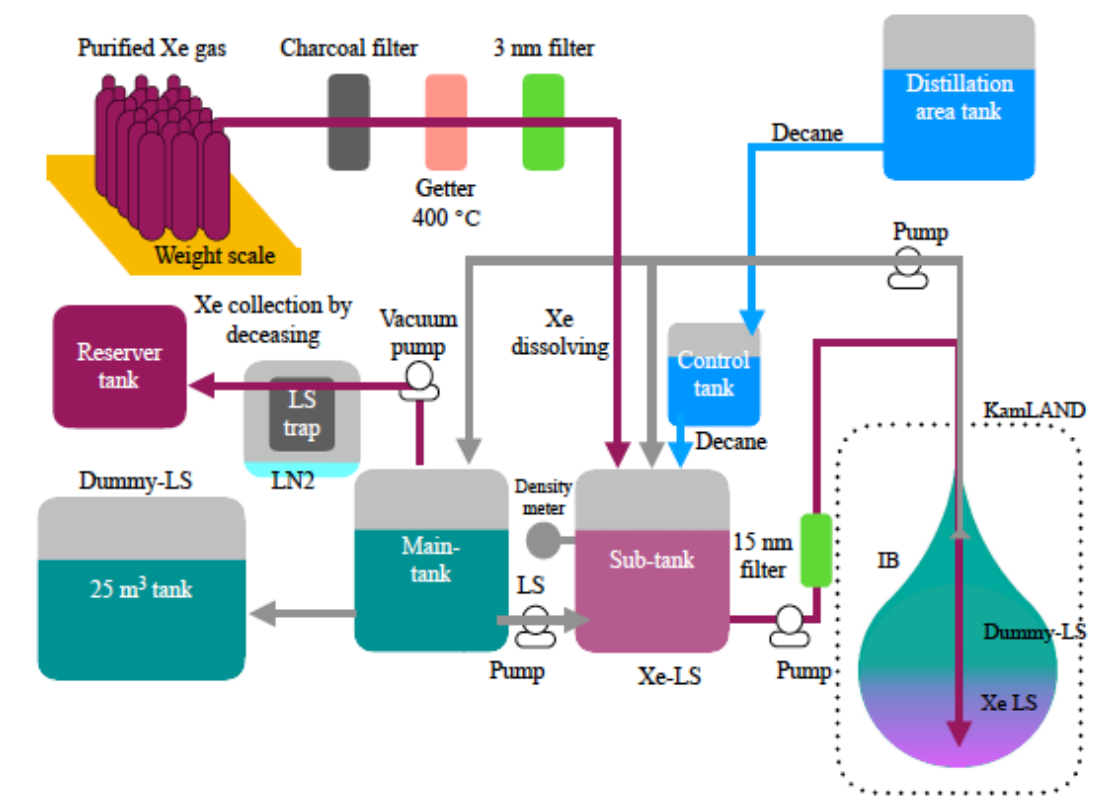
\includegraphics[scale=0.5]{xenonhandling.png}
	\caption{Flow diagram of the KLZ Xenon system. The purple lines denote the flow of Xe/XeLS, the blue line denotes the flow of decane, the the grey line denotes the flow of LS. Figure from Reference }
	\label{fig:xenonhandling}
\end{figure}

\section{Data Acquisition}
\subsection{KamLAND DAQ}
KamLAND uses two data acquisition (DAQ) systems in parallel. The first is KamFEE (KamLAND Front End Electronics), which has been used since the start of KamLAND physics data-taking. The other is MoGURA (Module for General-Use Rapid Application). MoGURA is a data acquisition system developed to eliminate the deadtune just after cosmis ray muon events. An overview of this dual scheme data acquisition system is shown in \ref{fig:kamland_daq}. What follows is a brief description of each DAQ system.
\subsection{KamFEE DAQ}
KamFEE are the front end electronics that read and control the KamLAND PMTs. The boards are of VME 9U form factor and are synchronized with a 40 MHz clock. The PMT signals are sent along two parallel channels. The first channel is sent to a discriminator which register a PMT hit if the voltage exceeds a predetermined value that corresponds to approximately 1/6th of a single photoelectron. The second channel, is delayed to give some time to process the discriminator signal and is fed into 3 amplifier stages (x20, x4, x0.5), this amplified signal is digitized by two analog Transient Waveform Digitizers (ATWDs). The ATWD is a 10-bit digitizer and samples every 1.5ns, 128 times per waveform. Each pulse takes 128 $\mu$sec to digitize.

The KamFEE boards send a "hitsum" signal to the central KamFEE DAQ trigger, communicating a certain number of hits were received and can be digitized. The trigger board sends a signal back which issues the digitization command to the ATWDs. While the ATWD is digitizing, it cannot record further signals, therefore, two ATWDs are assigned to each channel to reduce deadtime.

\subsection{MoGURA}
MoGURA is the secondary data acquisition system in KamLAND; it is responsible for after pulses and dealing with PMT waveform overshoots caused cosmic muons. KamLAND has a cosmic muon rate of 0.3 Hz, so it is important to compensate for the effects these high-energy events have on our detector. To accomplish this task, MoGDAQ has a few extra features over KamFEE.
\begin{itemize}
	\item \textbf{Baseline Recovery:} After a high energy muon passes through the detector, the DAQ channels are saturated, which means the voltage exceeds the digitization window, so only the maximum value is read. Simultaneously, the voltage "overshoots" as it returns to normal and swings below the nominal value causing difficulties in digitizing signals that occur soon after these muons. 
	\item \textbf{Adaptive mode:} Activates a special trigger mode after muon events to compensate for large after-pulses post-muon. This special trigger is based on differential PMT hits. 
\end{itemize}

MoGURA data is used to tag neutrons created from muon spallation. These tagged spallation neutrons are vital in subsequent analyses to tag events that likely originated from these cosmic ray muons. The baseline restoration and neutron tagging will be further improved with the implementation of MoGURA2 trigger system. This is a planned replacement of the KamLAND data acquisition system (KamFEE and MoGDAQ both) for the KamLAND2-ZEN experiment, which is planned to begin physics data-taking in 2028.

\section{KamLAND-ZEN Phases}
The KamLAND-ZEN experiment has undergone multiple phases and renovations.
\subsection{KamLAND-ZEN 400}
The inner balloon and XeLS was added to the KamLAND experiment in 2011, starting the phase referred to as KamLAND-ZEN 400. This phase of the detector featured a 3m diameter inner-balloon filled with liquid scintillator loaded with 3\% Xenon by weight. The dissolved Xenon gas had 91\% proportion of Xe$^{136}$.

The KamLAND-ZEN 400 data was split into two data-taking periods. Period-I data was contaminated with a high background of Ag$^{110m}$, the silver appeared to be leeching from the mini-balloon into the XeLS. The Ag$^{110m}$ contamination on the inner balloon was likely due to nuclear fallout from the Fukushima reactor meltdown. The Fukushima meltdown occurred when the inner balloon was being manufactured and in the same geographical region of Japan. Period II started after the XeLS distillation suppressed the Ag$^{110m}$ by a facator of 20. Period II continued data taking for 534.5 total livedays and the combined physics result of Periods I and II produced a \0nbb half-life limit of $T_{1/2}^{0\nu}>1.07\times 10^{25}$ years at 90\% C.L. This half-life limit corresponds to an effective majorana mass limit of $m_{\beta\beta} < 61-165$ meV. 
\subsection{KamLAND-ZEN 800}
KamLAND-ZEN 800 was the second phase of KamLAND-ZEN. KamLAND-ZEN took data from January 2019 to August 2024. Over 2kton$\cdot$yrs of exposure was observed. KamLAND-ZEN 800 was decommission in Fall 2024, and is currently being dissassembled. \\
\textbf{Inner Balloon Manufacturing}\\
KamLAND-ZEN 800 featured a larger, cleaner inner balloon which was fabricated at Tohoku University in a Class 1 cleanroom. The inner balloon is made from panels of 25 $\mu$m nylon-6. Innerballoon fabrication consisted of multiple steps some of these critical steps are listed here:
\begin{itemize}
	\item \textbf{Washing} - the film is cleaned twice in an ultrasonic bathtub, then stored between cover films to prevent dust adhesion
	\item \textbf{Welding} - the cleaned balloon panels are welded with a semi-automatic welding machine. For delicate areas, such as the balloon neck, a hand welding machine was used. The average tensile strength on the balloon surface was 35 $N/cm$ after welding.
	\item \textbf{He Leak Check} - Inevitably leaks will occur during the previous assembly procedures. Helium gas was pumped into the balloon to check for these leaks. The cover film of the balloon was peeled off before this leak check. Found leaks were repaired by patching the film. Over 900 leaks were found during the leak check.
	\item \textbf{Folding} - The inner balloon was folded into a cylinder shape and covered with sheath films to prevent contamination during transport. Teflon sheets and Vectran strings were used to tie the rolled balloon up for shipping.
	\item \textbf{Shipping} - The inner balloon was shipped within a silver gas bag. All corresponding tools were also shipped in airtight bags.
\end{itemize}
The inner balloon was installed on May 10, 2018. A rehearsal installation was performed in a swimming pool before the final deployment. In the final installation, the balloon is deployed through the 50cm port on the neck of the KamLAND detector. After filling the balloon with KamLS, the Teflon sheets, sheath films, and Vectran strings are pulled out of the detector. The whole operation was monitered in real-time via cameras and endoscope.

The top of the inner balloon is connected to a corrugated tbue made from PEEK (poly-ether-ether-ketone). Twelve suspending belts support the inner balloon, wrapping around the full height of the balloon. The tension of each of these belts are monitored in real time to guarantee the position and stability of the balloon. A schematic of the balloon structure can be seen in Figure \ref{fig:balloon_structure}. 
\textbf{Contamination Control}\\
Once deployed and exposed to the KamLAND scintillators, the inner balloon is very difficult to clean. Thus, maintaining balloon cleanliness is vital. After deployment, the IB was filled with distilled LS while the $^{232}$Th level was measured at $10^{-15}$g/g, exceeding the target background concentration. The PPO distillation tower was suspected to be a source of contamination and was investigated. ICP-MS and neutron activation analysis were used to measure $^{232}$Th contamination at different locations along the distillation system. After meticulous washing and filter replacement, LS purification began to lower the $^{232}$Th background. After two separate distillation campaigns, $^{238}$U and $^{232}$Th levels were reduced by a factor of 10 compared to KamLAND-ZEN 400. The contaminations can be estimated by performing a $^{214}$Bi-$^{214}$Po and $^{212}$Bi-$^{212}$Po coincidence analysis. The coincidence event rates plotted over time are shown in Figure and listed in Table.

KamLAND-ZEN 800 was decomissioned in 2024 after observing over 2 kiloton$\cdot$yrs of exposure. The final half-life limit was reported as $T_{1/2}^{0\nu} > 3.8\times 10^{26}$ years at 90\% C.L. This half-life limit corresponds to an effective majorana mass limit range of 28-122 meV. As of Summer 2025, this is the world-leading limit on effective majorana mass from any double-beta decay isotope and is the only limit in the Inverted Mass Ordering region.

\subsection*{KamLAND2-ZEN}



% {\bf Important}: You will also be using a lot of citations. The format in this template follows the so-called APA style and looks as follows in the document body: \cite{lamport1985:latex}, \cite{Debr01}. There are no numbers in the list of references -- the list is sorted alphabetically according to the first author's last name.

% Other styles of references are allowed by the library as well, e.g., ``plain'' or ``'ieee'', which use numbers in square brackets both in the document body and in the list of references. In order to use another style of references, e.g., ``plain'', follow the steps below:
% %
% \begin{enumerate}
%   \item In ``thesis.tex'' file:
% 	\begin{itemize}
% 	  \item comment out the line ``$\backslash$usepackage\{apalike\}'' at the top of the file,
% 	  \item replace ``$\backslash$bibliographystyle\{apalike\}'' with ``$\backslash$bibliographystyle\{plain\}'' towards the bottom of the file.
% 	\end{itemize}
%   \item In ``bu\_ece\_thesis.tex'' file, comment out all lines in the BIBLIOGRPAHY section (lines 503-517) and save it!
%   \item Recompile ``thesis.tex'' twice
% \end{enumerate}

